In this section, we take a close look at the proposed structure and capabilities of the framework's API.
The final implementation will however deviate with a high probability.
The final paper will be corrected to account for these changes\footnote{TODO: Tamino, might also want to check with Marc.}.

\section{Proposed Functionality}

The framework shall have two primary capabilities: first, it should enable fast and easy access to the 3d space calculated from the marker.
Second, given a model to display, it should be capable of returning a rendering of the object within the scene.

Generally, the framework shall work as in the following.
Upon import of the framework into the project, the program passes the image to the framework.
This shall be possible to do in two ways: one, let OpenCV read directly from the camera, or two, give the framework the frames from the program manually.
This allows the possibility of using other video or picture streams with the framework\footnote{For example, rendering an object into a video.}.

Now the magic happens; OpenCV calculates the 3d space.
Before passing it on to the framework, the program can read the 3d space.
This direct access to the resulting coordinate space allows a more down-to-earth programming should it be required.
If the program is only interested in the final rendered frame, given a model, the framework then renders the object into the scene and returns the frame to the program.

Apart from the above mentioned basic functionality capabilities, the framework should also handle the easy gathering of performance and error information.
Accessing the information will be done via a listener or an equal mechanism so that any developers can choose when and how to use the information collected by the framework.
Care should be taken to ensure that the error collection can run even when the framework encounters problems, possibly by putting it in a separate thread.

\begin{figure}
	\centering
	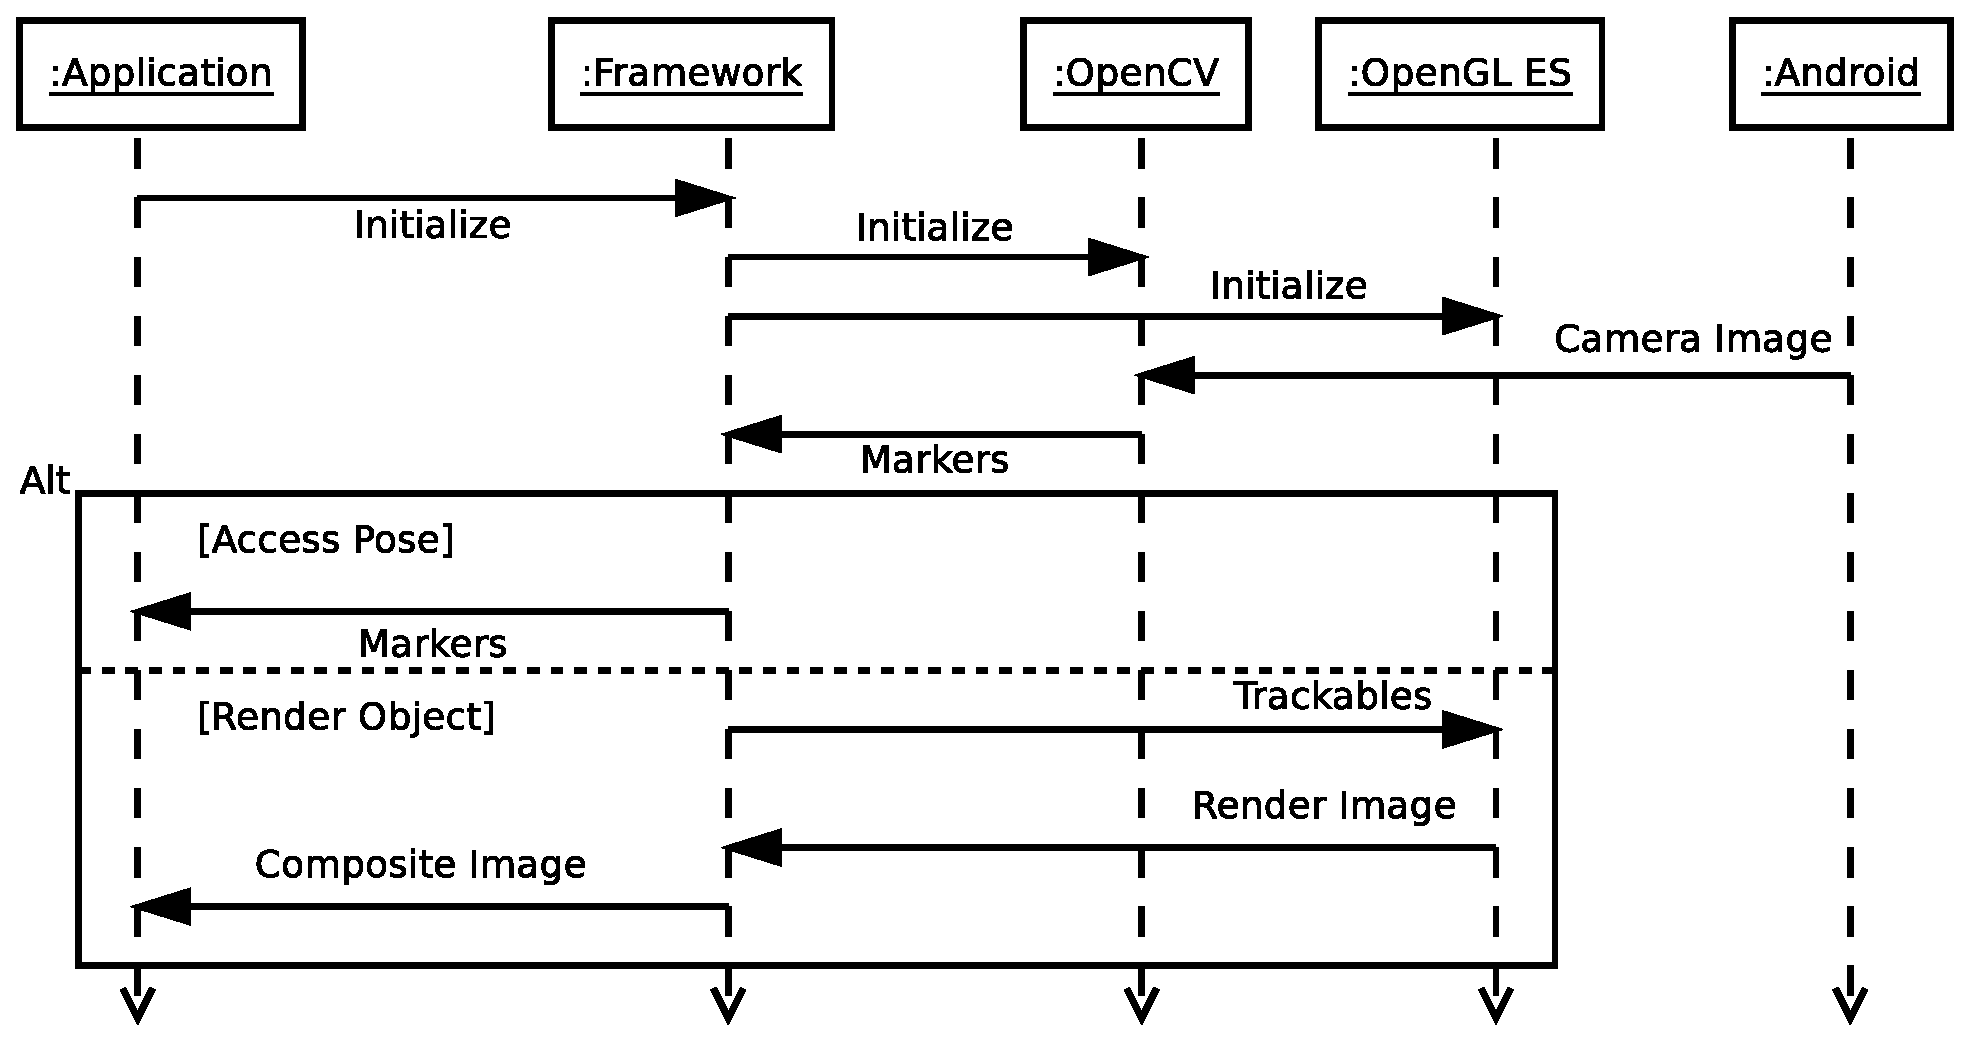
\includegraphics[width=12cm]{img/sequence_access.eps}
	\caption[Access Sequence.]{The proposed sequence of the workflow with the framework, using OpenCV.}
	\label{fig:sequence_access}
\end{figure}

Figure \ref{fig:sequence_access} shows the proposed outside view of the framework, and where data can be input or read.
As proposed, the framework should offer a wide variety of uses, without being overly complex.
Another important aspect we want to make possible is the possibility of changing all the more important parameters during runtime, such as switching the model or adding a new marker.
This should allow a much smoother usage of the framework and any derived apps as a result.

\section{Dependencies}

The framework will depend on two external software solutions.
The first is OpenCV, an open source collection of computer vision and machine learning software.
For this work, we implement it's API.
To use the framework on Android, the OpenCV Manager\footnote{See: \url{https://play.google.com/store/apps/details?id=org.opencv.engine}.} needs to be installed.
This program offers the best version for each Android device according to its specifications and capabilities.
Apart from OpenCV, OpenGL ES 2.0 is used for the rendering of the 3D objects to the display.

TODO: Add OpenGL 2.0 stuff that might be important. Why not use 1.1 etc...

\section{Limitations of Scope}

To clarify the scope of the proposed framework, all features that will be delivered are described within the following table.
Note that while these are the main features, aspects of them might change for the implementation.

\begin{tabulary}{\textwidth}{L || L}
Debug Messaging & The framework should be easy to debug and allow simple access to status messages.\\
\hline
Manage Trackers & Allow to add and remove trackers during runtime.\\
\hline
Manage Rendering & Offer the possibility of putting an own render module into the pipeline and modify any properties required to render such as transparency, etc.\\
\hline
Read Raw Data & Give the possibility of accessing the raw data returned from the OpenCV Wrapper so that custom solutions can be built without changing the source code.\\
\hline
Modular Source Data & The source data should not be dependent on a certain device; using any video or image files as source should work equally well, if desired.
\end{tabulary}

The features in the following table are features that might be implemented, if their development proves to be beneficial to the framework and are easy enough to be added along the sidelines.

\begin{tabulary}{\textwidth}{L || L}
Animated Objects & Allow the object to have an animation and offer control access to it.\\
\hline
Simple Advanced Rendering & Possibly add some simple extra rendering features.\\
\end{tabulary}

The following are features that will not be implemented.
However, where possible, the framework will allow easy adaption to extend its functionality beyond what it will offer from the start.

\begin{tabulary}{\textwidth}{L || L}
Marker-less Tracking & Marker-less tracking will most likely not be within the scope of the initial framework. However, as changing markers during runtime will probably be possible, adding this feature should not be overly difficult.\footnote{TAMINO TODO: Might want to reword that.}\\
\hline
Occlusion & The capability to detect where scene occlusion is taking place is definitely beyond the scope of the framework, as this requires extensively more work.\\
\hline
Fancy Rendering & For now, no support of stereoscopic rendering of any kind. Depending on the difficulty of implementation, support for different direct rendering engines within the framework might be included which would allow an easy way of adding this functionality.\\
\end{tabulary}

\section{Class Diagram}

\begin{figure}
	\centering
	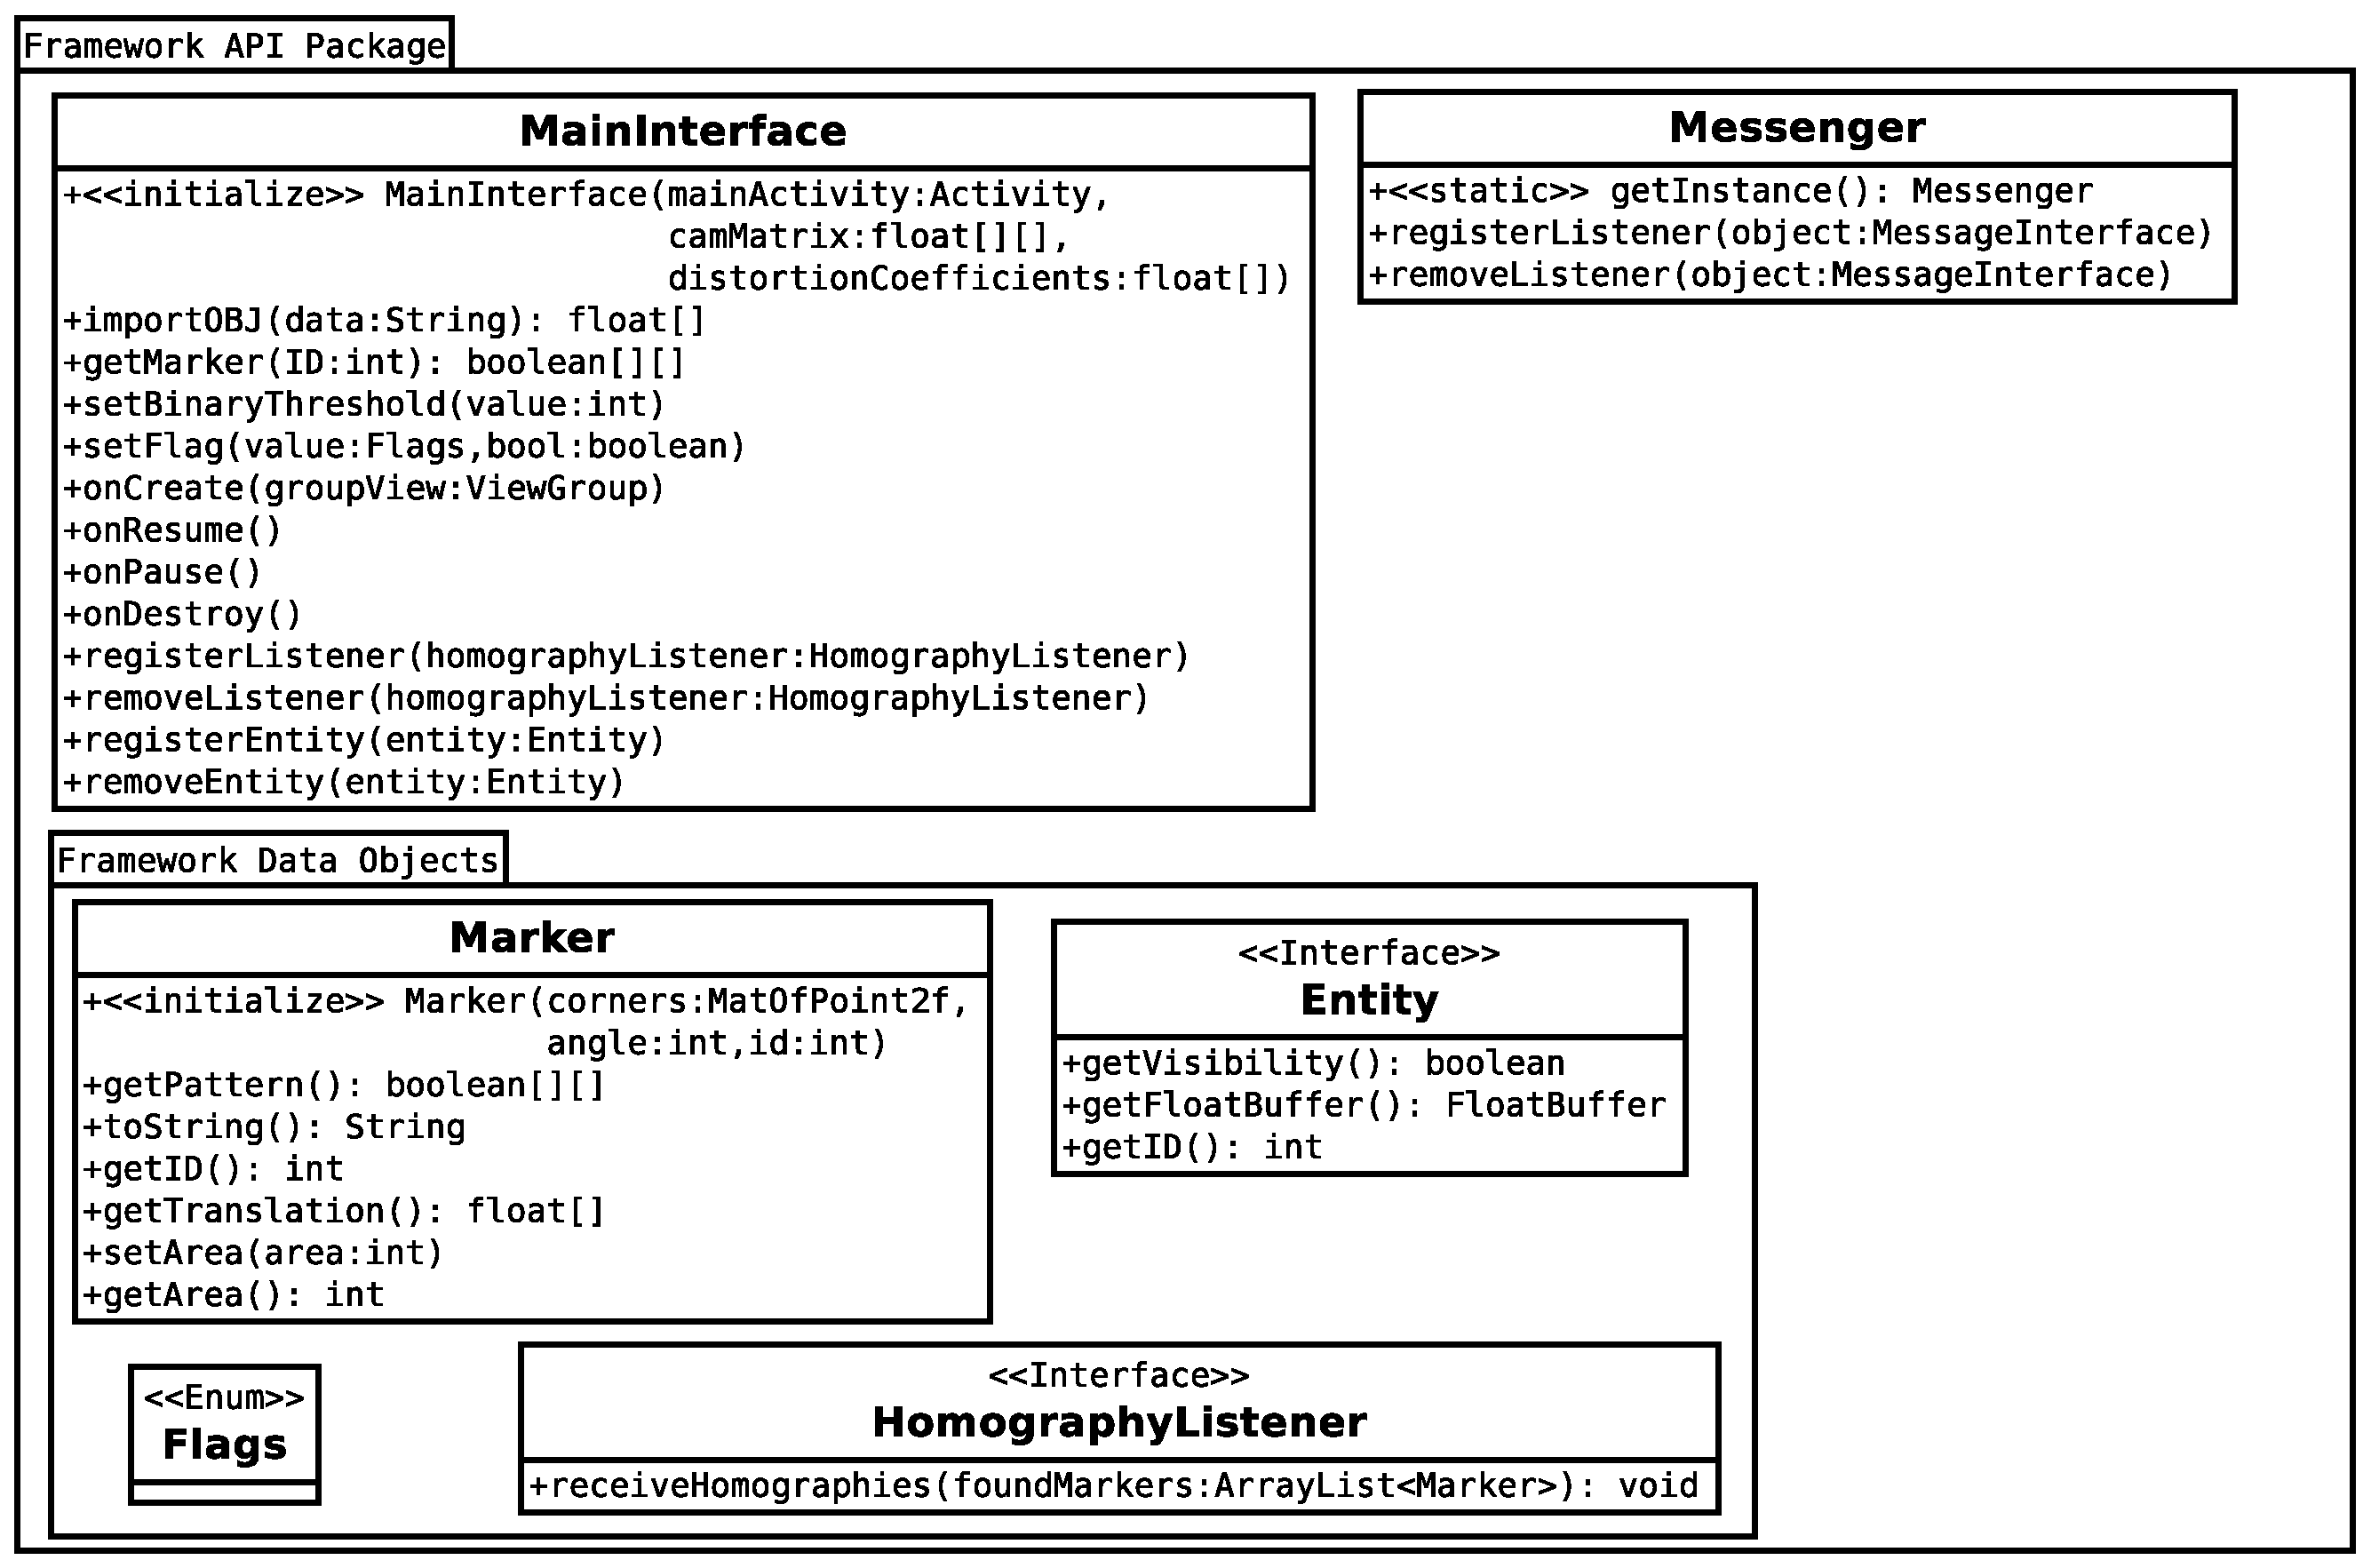
\includegraphics[width=10cm]{img/class_diagram.eps}
	\caption[General Class Diagram]{This is the preliminary class diagram of the proposed functionality of the framework. Note the low number of public methods: this should make usage of the framework very easy. Also note that the Messenger class has no dependencies towards other classes to enable it to run as a distraction-free subthread from the rest of the framework.}
	\label{fig:class_diagram}
\end{figure}

Now let us take a look at the proposed class structure within the framework, as seen in Figure \ref{fig:class_diagram}.
Main access is controlled over the framework controller, which almost exclusively contains all the public methods callable from outside of the framework.
Only the messenger class offers public access too.

The messenger class allows easy and quick access to any debugging, logging, or error messages to outside classes via a listener principle.
Allowing outside threads to be directly notified when a message is written enables comparatively fail-safe information gathering.
This should also help with the transparency of using the framework.
Note that to keep the messenger thread-safe, the register and remove methods for listeners are one atomic protected block.
The messenger thread itself is controlled from the framework with default behavior enabled should it stop running.

The Controller encapsulates all the primary functionality within the framework.
Apart from managing all the other classes on startup and closure, it also handles the information exchange between them and the caller.
It also enables the management of the trackables and their assigned renderables.
Changing the source for the video to detect markers and changing the rendering engine can be done here too, if desired.
The Controller also handles any inter-system compatibility that the passage of information between the Renderer and Wrapper require.

The OpenGL ES Renderer class handles the generation of the images for the output in the form of a canvas.
It takes the 3d coordinate system from the OpenCV wrapper and renders the objects with the given specifications onto the final canvas.

Last is the OpenCV Wrapper. The Wrapper handles the control of the OpenCV library and does any managing work required for the framework.
It also enables some source and destination control for respectively the images and 3d coordinate space.

The above proposed system should enable an easily extensible build for the framework.
For example, using the framework with any OpenCV version apart from the Android port should be achievable by simply writing an extra wrapper.
The same applies for the Renderer; it can simply be replaced by new modules that render to DirectX or the full OpenGL specification.
While we encourage such modularity, we will not promise it for the final version of this work.

\section{Application Programming Interface}

The following represents the suggested interface for the framework.
With the listed methods, all functionality that the framework offers can be accessed.

TAMINO TODO: Place javadoc here.

\section{Usage}

\begin{figure}
	\centering
	
\includegraphics[width=4cm]{img/marker_example.png}
	\caption[Example Marker.]{An example of a marker. This image is either printed or displayed by some other means in the real world to allow a system to use it as a reference to base a virtual overlay off of it.}
	\label{fig:marker_example}
\end{figure}

To enable the framework to detect a 3d coordinate system from a video feed, a marker with specific properties will be required.
A marker is a visually significant pattern that the system can detect within an image and be used to calculate spatial coordinates. Figure \ref{fig:marker_example} shows an example for such a marker.

TODO: Maybe add a small exposition about markers? See paper.

Depending on the capabilities of the finished framework, it could be possible to track multiple markers in a single instance.
This would allow multiple objects to be rendered simultaneously, increasing the use cases for the framework – although care will have to be taken to keep any overhead to a minimum.

To enable the functionality, the recorded or live video stream must have a pre-defined marker somewhere in it.
This can be a screen showing the marker, a printed marker, or any other way of displaying a marker in a scene.
Depending on the capabilities of OpenCV, the framework will then detect its relative 3d position.
With the detected space, the framework can now render objects into the scene with the correct rotation, scaling, and perspective.

The framework should be made to be thread safe.
Internally the framework will most likely at least have one sub thread for error and information collection and propagation.
If possible, it should be easy to put the framework into its own thread domain so that any programs using it do not have to worry about locking down their threads by accessing the framework.
This means that the framework will most likely work asynchronous, with the possibility of forcing it to run synchronous where required.

\section{Implementation}

The following section describes in more detail the implementation of the framework.
First we implemented a test project to experiment with OpenCV on Android to collect data on possible solutions and problems.

At first, a feature-based approach was tried.
That meant that feature detection was used on the marker, resulting in a cloud of key feature points.
These can then theoretically be located in an image from which we have likewise extracted feature points.
However, this method proved to be too computationally expensive.
Initial tests only for detecting feature points in a live camera view already yielded framerates below 2 frames per second.
This was deemed insufficient for a realtime use of the finished product.

More research turned up a better solution based on the method used by the comparable Aruco\cite{aruco} framework.
The method was implemented as follows.

\subsection{Method for Tracking Markers}

The following is done each frame with OpenCV.
It results in a list of detected markers with their transformation matrices.

First, the input frame is transformed into a simple gray-scale image.
This gray-scale image is then processed with the Canny\cite{canny} edge detector, resulting in nice continuous edges of most objects within the frame.
We then extract all contours from the edges.
These contours are used to fit polynomial approximations to all detected contours.
We can then filter the polynomial objects based on criteria for our markers, mainly for any contours that have 4 corners and conform to certain angles.
These filtered contours are then processed to identify which marker is which contour.

One of the major advantages of the polynomial representation of the markers is that it allows easy extraction of the homography required to calculate the 3d position of the markers.
Apart from that, it is also significantly faster – our first tests resulted in framerates of about 8 frames per second.

However, while 8 fps is better than 2 fps, it is still somewhat too slow for easy use.
Therefor, we suggest using multitasking to process multiple frames in parallel.
Some optimizations that we also use include writing all the OpenCV calls in a single, native C++ method that is called from the Java framework.
That call is also the point where the framework can easily be adapted to different systems, as switching the OpenCV calls can easily be done by writing a new, comparable method that simply replaces that single call.

\section{How to Use}

Using the framework is very easy.
Simply create an instance of the MainInstance of the framework either in the constructor or in the onCreate method.
After creating the instance, call the onCreate method of the framework within the activity's onCreate.
To create the framework, it requires an Android GroupView where it will place the camera view and the view responsible for rendering the detected objects.
Now all that remains is to also call onPause, onResume, and onDestroy in the respective functions of the activity via the framework.
Now the parameters of the framework can be changed at any time, probably with event listeners.
